\documentclass{article}
\usepackage{hyperref}
\usepackage{listings}
\usepackage{color}
\usepackage{xcolor}
\usepackage{geometry}
\usepackage{graphicx}
\usepackage{amsmath}
\usepackage{caption}
\usepackage{subcaption}
\geometry{margin=1in}
\pdfminorversion=6

\newcommand\TODO[1]{\textcolor{red}{TODO: #1}}

\newcommand\header[2]{
    \begin{center}
        {\large
        UCSD CSE 168 Assignment #1: \\
        \vspace{0.3cm}
        \Large
        #2}
    \end{center}
}

\definecolor{dkgreen}{rgb}{0,0.6,0}
\definecolor{gray}{rgb}{0.5,0.5,0.5}
\definecolor{mauve}{rgb}{0.58,0,0.82}
\lstset{frame=tb,
        aboveskip=3mm,
        belowskip=3mm,
        showstringspaces=false,
        columns=flexible,
        basicstyle={\small\ttfamily},
        numbers=none,
        numberstyle=\tiny\color{gray},
        keywordstyle=\color{blue},
        commentstyle=\color{dkgreen},
        stringstyle=\color{mauve},
        breaklines=true,
        breakatwhitespace=true,
        tabsize=2
}

\hypersetup{colorlinks=true}

\usepackage{xcolor}

\begin{document}

\header{3}{Indirect lighting, BRDFs, and Multiple Importance Sampling}
In this homework, we will implement an actual \href{https://en.wikipedia.org/wiki/Path_tracing}{path tracing} algorithm. We will finish the RTRYL book this time!

\section{Diffuse interreflection}
So far in our code, we seem to be treating the diffuse and specular surfaces separately: diffuse surfaces gather contributions from lights, and specular surfaces trace out rays that collect color from other surfaces (and \lstinline{plastic} is a mixture of them). In real world, diffuse surfaces also collect colors from other surfaces. We will implement this in this part.

In the previous homeworks, we do something like this:
\begin{lstlisting}[language=python]
def radiance(scene, ray, rng):
  if (ray intersect scene):
    # [emission] add emission of the intersected shape
    # ...
    # [direct_lighting] loop over lights, sample them, and sum over their contributions
    # ...
    # [scattering] recursively tracing the ray by calling radiance
    if (hit a metal or plastic):
      # recursively trace a ray towards the mirror reflection direction
      # ...
  else:
    return scene.background_color
\end{lstlisting}

In this homework, we will temporarily suspend the direct lighting code -- we will add it back later in the next homework.

We will extend the scattering code to handle diffuse materials in this homework. As with the case of area light, conceptually this is simple: instead of always tracing rays towards the mirror reflection direction, we randomly sample rays at different directions and accumulate contributions (\href{https://raytracing.github.io/books/RayTracingInOneWeekend.html#diffusematerials}{Chapter 8} of RTOW describes one approach to do this). But what distribution should we use, and how do we weigh different directions? That's where we need to do the math.

Remember the area light integral, where we integrate over all points on a light source $S$:
\begin{equation}
\int_{x \in S} f(x) \mathrm{d}A(x) = \int_{x \in S} \frac{K_d \cdot \max\left(n_s \cdot l, 0\right)}{\pi} \cdot \frac{I \max\left(-n_x \cdot l, 0\right)}{d^2} \cdot \text{visibility} \cdot \mathrm{d}A(x),
\label{eq:area_light}
\end{equation}
where $K_d$ is the diffuse reflectance, $n_s$ is the normal at the shading point, $l$ is the unit vector pointing from the shading point towards $x$, $n_x$ is the geometric normal at point $x$ on the light source, and $d$ is the distance between the shading point and $x$.

We will derive the equations of diffuse interreflection from Equation~\eqref{eq:area_light}. Let's play with an idea: what if everything is light source? We will figure out how to assign the intensity $I$ later. Apart from the intensity, all we need to change is the integration domain: instead of integrating a particular light source $S$, we integrate over all surfaces $\mathcal{M}$. Next, since we are tracing rays, we want to deal with directions, instead of points on surfaces. We achieve this using a \emph{change of variable} (again!) -- instead of integrating over position $x$, we integrate over (outgoing) direction $\omega_o$:
\begin{equation}
\int_{x \in \mathcal{M}} \frac{K_d \cdot \max\left(n_s \cdot l, 0\right)}{\pi} \cdot \frac{L \max\left(-n_x \cdot l, 0\right)}{d^2} \cdot \text{visibility} \cdot \mathrm{d}A(x) = 
\int_{\omega_o \in \Omega} \frac{K_d \cdot \max\left(n_s \cdot \omega_o, 0\right)}{\pi} \cdot L \cdot \mathrm{d}\omega_o.
\label{eq:area_light_solid_angle}
\end{equation}
Firstly, we have replaced $S$ with $\mathcal{M}$ and $I$ with $L$ to emphasize that things are different now.
Also note that $\omega_o = l$.
Here, the measure $\mathrm{d}\omega_o$ is often called the \href{https://en.wikipedia.org/wiki/Solid_angle}{solid angle} -- it represents an infinitesimal area of a point on a unit sphere. You will notice that the equation gets a lot simpler after we switch to the solid angle measure. This is because the Jacobian of the change of variable is exactly the reciprocal of $\frac{\max\left(-n_x \cdot \omega_o, 0\right)}{d^2} \cdot \text{visibility}$ (see \href{https://raytracing.github.io/books/RayTracingTheRestOfYourLife.html#samplinglightsdirectly/gettingthepdfofalight}{Chapter 9.1} of RTRYL for an explanation). Intuitively, the Jacobian captures the ratio of area on the surface $\mathcal{M}$ and its projcted area on a unit sphere (if it is not blocked).

We still need to decide what is the color $I$. Remember in the mirror case, we recursively trace rays to determine the color. We can do the same thing for diffuse surfaces too!
\begin{equation}
L = \int_{\omega_o \in \Omega} \frac{K_d \cdot \max\left(n_s \cdot \omega_o, 0\right)}{\pi} \cdot L \cdot \mathrm{d}\omega_o.
\end{equation}
This is however vacuous, because there is no \emph{base case} for this recursion. We will instead add the emission whenever we hit a light source\footnote{The infinite recursion defined in Equation~\eqref{eq:diffuse_rendering_equation} is actually mathematically well-behaved, as long as $K_d < 1$ for all channels. The reason is that after each bounce, some energy will be absorbed by $K_d$, and eventually the ray will carry zero energy.}:
\begin{equation}
L = L_e + \int_{\omega_o \in \Omega} \frac{K_d \cdot \max\left(n_s \cdot \omega_o, 0\right)}{\pi} \cdot L \cdot \mathrm{d}\omega_o.
\label{eq:diffuse_rendering_equation}
\end{equation}
We have arrived at the (in)famous \href{https://en.wikipedia.org/wiki/Rendering_equation}{rendering equation} (though specialized at diffuse BRDFs).

Now, we need to sample a direction $\omega_o$ for evaluating the integral in Equation~\eqref{eq:diffuse_rendering_equation}. For this, read \href{https://raytracing.github.io/books/RayTracingTheRestOfYourLife.html#lightscattering}{Chapter 5-8} of RTRYL. We will implement the cosine hemisphere sampling described in the book. You do not need to implement the light sampling yet (Chapter 9). You also only need to handle diffuse materials. We will add light sampling and other materials back later!

Go to the function \lstinline{hw_4_1} in \lstinline{hw4.cpp} and implement diffuse interreflection using cosine hemisphere sampling. The function also takes an extra command line parameter \lstinline{-max_depth [max_depth]}, which you will use to limit the maximum recursion depth of your path tracer. 

To test your results, type:
\begin{lstlisting}[language=bash]
./torrey -hw 4_1 ../scenes/hw1_spheres/scene0_spherical_light.xml
./torrey -hw 4_1 ../scenes/cbox/cbox.xml
./torrey -hw 4_1 ../scenes/party/party_bgonly.xml
./torrey -hw 4_1 ../scenes/sponza/sponza_bgonly.xml -max_depth 6
./torrey -hw 4_1 ../scenes/living-room-Wig42/scene_bgonly.xml
\end{lstlisting}

\paragraph{Energy conservation.} Remove the $\frac{1}{\pi}$ in Equation~\eqref{eq:diffuse_rendering_equation} and render the \lstinline{cbox} scene again (you still need to have the $\pi$ in your PDF since PDFs need to integrate to $1$). What do you observe? Why?

See Figure~\ref{fig:hw_4_1} for the references. You can notice that the images are much more noisy this time. I did not run all of them to convergence since it's starting to take a while to render (even so, these images can already take tens of minutes to render!). If you run them overnight (with, say, 10000 samples per pixel), you should see relatively clean images. Since we are relying on randomly trace light path until we hit a light source, the chance that it hits a light can often be small. The light sampling we will implement later helps with this, but it would not fully solve the problem as we have very large light sources in these scenes. This is why there are active research projects on trying to make rendering faster -- it's hard! Modern renderers will likely apply \href{https://cgg.mff.cuni.cz/~jirka/path-guiding-in-production/2019/index.htm}{path guiding}, \href{https://cs.dartmouth.edu/~wjarosz/publications/bitterli20spatiotemporal.html}{importance resampling} and \href{https://www.cmlab.csie.ntu.edu.tw/project/sbf/}{denoising} to speedup the rendering. These could be cool final projects if you are interested.

Another thing to notice is that how the global illumination automatically make the images look significantly more realistic! By physically simulating lights, we are able to automagically create realistic images without much efforts. Before people start to simulate global illumination in their renderers, artists have to manually place lights and draw textures to approximate the effect, which is extremely time consuming -- now we just let computers spend that time! Even better, compared to recent learning-based generative models, the physically-based rendering approach still let us have full precise control of how the image looks like. We fully understand how the color of each pixel is generated, and we can change the way it is generated if we know how to write a renderer.

\begin{figure}[ht]
    \centering
    \includegraphics[width=0.20\linewidth]{imgs/hw_4_1a.png}
    \includegraphics[width=0.15\linewidth]{imgs/hw_4_1b.png}
    \includegraphics[width=0.20\linewidth]{imgs/hw_4_1c.png}
    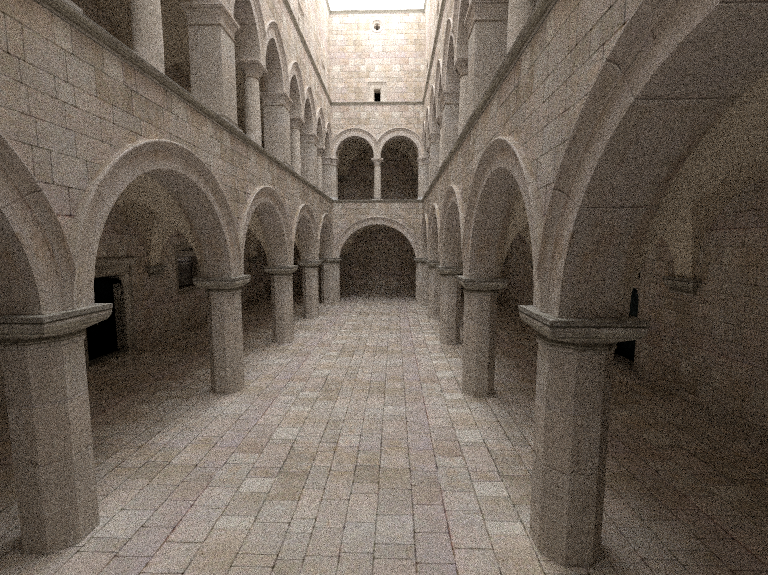
\includegraphics[width=0.20\linewidth]{imgs/hw_4_1d.png}
    \includegraphics[width=0.20\linewidth]{imgs/hw_4_1e.png}
    \caption{References for Homework 4.1.}
    \label{fig:hw_4_1}
\end{figure}

\section{Adding non-diffuse materials}
Let's add back \lstinline{mirror}, \lstinline{plastic}, and let's add more. 

\subsection{Adding back \protect\lstinline!mirror! and \protect\lstinline!plastic!}
Adding back \lstinline{mirror} should be easy, we will let you figure that out. Adding back \lstinline{plastic} is slightly more involved. Should we follow the diffuse sampling direction or the specular sampling direction? The answer is -- we choose them stochastically! Since the diffuse and specular components are weighted by the Fresnel term $F$, we roll a dice and trace the specular ray with probability $F$, and trace the difuse ray with probability $1-F$. To be more concrete, mathematically it works like this -- we have an expression:
\begin{equation}
L = F a + (1 - F) b.
\end{equation}
We want to use Monte Carlo sampling to evaluate this expression. We evaluate the first term with probability $F$, and the second term with probability $1-F$. Our Monte Carlo estimator is:
\begin{equation}
\left<L\right> = \begin{cases}
\frac{F a}{F} & \text{with probability } F \\
\frac{\left(1 - F\right) b}{1 - F} & \text{with probability } 1 - F
\end{cases}.
\label{eq:discrete_mc}
\end{equation}
If we take the expectation of $\left<L\right>$, we can see that it is an \href{https://en.wikipedia.org/wiki/Bias_of_an_estimator}{unbiased estimator}:
\begin{equation}
E\left[\left<L\right>\right] = F \cdot \frac{F a}{F} + (1 - F) \cdot \frac{(1 - F) b}{1 - F}.
\end{equation}
The same math works even if $a$ and $b$ are both Monte Carlo estimators themselves.

\paragraph{Quiz:} Let's consider the following, different estimator:
\begin{equation}
\left<\hat{L}\right> = \begin{cases}
\frac{F a + (1 - F)b}{F} & \text{with probability } F \\
\frac{F a + (1 - F)b}{1 - F} & \text{with probability } 1 - F
\end{cases}.
\end{equation}
Is it unbiased? Should we use this one or Equation~\eqref{eq:discrete_mc}?\footnote{If you love math, \href{https://ecommons.cornell.edu/handle/1813/13985}{Chapter 2.3} of Milos Hasan's thesis has some cool theoretical discussions on what is the best way to do this.}

Check your \lstinline{mirror} and \lstinline{plastic} renderings using the following scenes:
\begin{lstlisting}[language=bash]
./torrey -hw 4_2 ../scenes/hw1_spheres/scene1_spherical_light.xml
./torrey -hw 4_2 ../scenes/cbox/cbox_area_light_spheres.xml
\end{lstlisting}
Figure~\ref{fig:hw_4_2_mirror_plastic} shows our renderings of them.

\begin{figure}[ht]
    \centering
    \includegraphics[width=0.40\linewidth]{imgs/hw_4_2a.png}
    \includegraphics[width=0.40\linewidth]{imgs/hw_4_2b.png}
    \caption{References for \lstinline{mirror} and \lstinline{plastic} materials for HW 4.2.}
    \label{fig:hw_4_2_mirror_plastic}
\end{figure}

\subsection{Phong BRDF}
After you add back \lstinline{plastic}, let's add a few more materials. It feels weird that our rays either uniformly spread like a diffuse material, or it pinpoint at the mirror reflection direction -- there must be something in between! In general, instead of a cosine distribution multiplied by $\frac{K_d}{\pi}$, we can replace it with a general \emph{bidirectional reflectance distribution function} (BRDF) $\rho$\footnote{In many literatures, BRDF does not include the cosine term, but I find it cleaner to combine the both most of the time.}:
\begin{equation}
L = L_e + \int_{\omega_o \in \Omega} \rho \cdot L \cdot \mathrm{d}\omega_o.
\label{eq:rendering_equation}
\end{equation}

Designing a good BRDF $\rho$ is an active research topic. A simple BRDF, again goes back to the legedary \href{https://en.wikipedia.org/wiki/Phong_reflection_model}{Phong}, is to define a cosine falloff function around the mirror reflection direction\footnote{Some variants add a cosine term to the end, but I find that produces darkening appearance at grazing angles.}:
\begin{equation}
\rho_{\text{phong}} \propto \begin{cases}
K_s \max\left(r \cdot \omega_o, 0\right)^\alpha & \text{ if } n_s \cdot \omega_o > 0 \\
0 & \text{ otherwise} 
\end{cases},
\end{equation}
where $K_s$ is the reflectance color, $r$ is the mirror reflection direction, and $\alpha$ is usually called the \emph{Phong exponent} -- the larger it is, the sharper the distribution is. Notice that we only define the distribution up to a normalization constant. Choosing a proper normalization is important for BRDFs (why?). When Phong derived his reflection model, they did not have to worry about normalization because they were not doing path tracing. To use Phong's reflection model in our renderer, we need to derive a constant.

For a BRDF $\rho(\omega_i, \omega_o)$ to be energy conserving, it needs to satisfy the following condition:
\begin{equation}
\int_{\omega_o \in \Omega} \rho(\omega_i, \omega_o) \mathrm{d}\omega_o \leq 1 \text{ for all } \omega_i.
\end{equation}
Throughout this homework, we assume $\omega_i$ to be pointing \textbf{out} from the surface.
To ensure the Phong BRDF $\rho_{\text{phong}}$ satisfies this criterion, we need to choose a constant $C$ such that
\begin{equation}
C \cdot K_s \int_{\omega_o \in \Omega} \left(r \cdot \omega_o\right)^\alpha \mathrm{d} \omega_o \leq 1
\end{equation}
for any incoming direction $\omega_i$ ($r = -\omega_i + 2 n_s \left(n_s \cdot \omega_i\right)$). 
We find that the maximum of the integral is achieved when $\omega_i = n_s$. In such case, the reflection direction $r$ is also at the normal direction $n_s$:
\begin{equation}
K_s \int_{\omega_o \in \Omega} \left(r \cdot \omega_o\right)^\alpha \mathrm{d} \omega_o \leq K_s \int_{\omega_o \in \Omega} \left(n_s \cdot \omega_o\right)^{\alpha} \mathrm{d} \omega_o.
\label{eq:phong_inequality}
\end{equation}
The second integral in Equation~\eqref{eq:phong_inequality} has a closed-form. To see this, let's convert it to a spherical coordinate where the $z$-axis is the direction of $n_s$:
\begin{equation}
\int_{\omega_o \in \Omega} \left(n_s \cdot \omega_o\right)^{\alpha} \mathrm{d} \omega_o = 
\int_{0}^{2\pi}\int_{0}^{\frac{\pi}{2}} \left(\cos\theta\right)^{\alpha} \sin\theta \mathrm{d}\theta \mathrm{d}\phi = 
\int_{0}^{2\pi} \left. \frac{-1}{\alpha + 1} \left(\cos\theta\right)^{\alpha + 1} \right|_{\theta=0}^{\frac{\pi}{2}} \mathrm{d}\phi = \frac{2\pi}{\alpha + 1}.
\label{eq:phong_normalization}
\end{equation}
So, if we set $C = \frac{\alpha + 1}{2\pi}$, as long as $K_s \leq 1$, Phong BRDF always conserve energy:
\begin{equation}
\rho_{\text{phong}} = \begin{cases}
K_s \frac{\alpha + 1}{2\pi} \max\left(r \cdot \omega_o, 0\right)^\alpha & \text{ if } n \cdot \omega_o > 0 \\
0 & \text{ otherwise.} 
\end{cases}
\label{eq:phong}
\end{equation}

Sampling the Phong BRDF isn't that different from sampling the diffuse BRDF. We first sample the cosine lobe ($\max\left(r \cdot \omega_o, 0\right)^\alpha$) assuming the mirror reflection direction $r$ is facing towards $z$. Then we build an orthonormal basis with the $z$ axis pointing towards the mirror reflection direction. We then use the orthonormal basis to transform the local 3D vector to the mirror reflection direction basis.

To importance sample the local cosine lobe, we turn into spherical coordinates and define the PDF we want to sample from:
\begin{equation}
\mathbf{p}_{\text{phong}}(\theta, \phi) \propto \left(\cos\theta\right)^{\alpha} \sin\theta.
\end{equation}
From Equation~\eqref{eq:phong_normalization}, we already know that the normalization factor of this PDF:
\begin{equation}
\mathbf{p}_{\text{phong}}(\theta, \phi) = \frac{\alpha + 1}{2\pi}\left(\cos\theta\right)^{\alpha}.
\end{equation}

\paragraph{Quiz:} Apply inverse transform sampling to derive the sampling procedure for the PDF above. Show your derivation process.

From $\theta$ and $\phi$, we come up with the local direction. We can then convert this local direction to the coordinate basis defined by the mirror reflection direction $r$. This conversion is also a change of variable, and we normally have to account for the Jacobian of this coordinate transformation. Interestingly, because the coordinate basis is orthonormal, the conversion has an Jacobian of $1$, so we do not need to account for the Jacobian.

Now, add the Phong BRDF (Equation~\eqref{eq:phong}) into your \lstinline{hw_4_2} code. A Phong BRDF of a scene is stored in the following format:
\begin{lstlisting}[language=C++]
struct ParsedPhong {
    ParsedColor reflectance; // Ks
    Real exponent; // alpha
};
\end{lstlisting}

We provide yet another Cornell box scene (yes, I am uncreative) and two other scenes for you to test your code:
\begin{lstlisting}[language=bash]
./torrey -hw 4_2 ../scenes/cbox/cbox_area_light_spheres_phong.xml
./torrey -hw 4_2 ../scenes/teapot/teapot_textured_phong.xml
./torrey -hw 4_2 ../scenes/teapot/teapot_textured_phong_grazing_view.xml
\end{lstlisting}
Our rendering of the scene is in Figure~\ref{fig:hw_4_2_phong}.

\begin{figure}[ht]
    \centering
    \includegraphics[width=0.45\linewidth]{imgs/hw_4_2c.png}
    \includegraphics[width=0.225\linewidth]{imgs/hw_4_2d.png}
    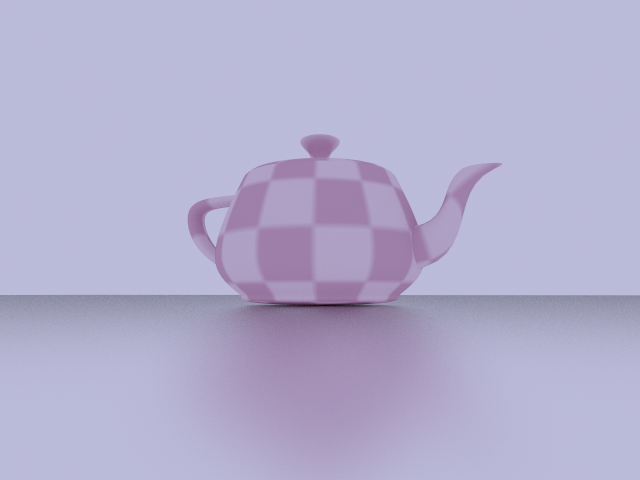
\includegraphics[width=0.225\linewidth]{imgs/hw_4_2e.png}
    \caption{Reference for the \lstinline{phong} materials for HW 4.2. For the left most scene, the Phong exponents are 100, 40, 8, 1, from left to right. For the middle and right scenes, the Phong exponent is 50.}
    \label{fig:hw_4_2_phong}
\end{figure}

\subsection{Blinn-Phong BRDF}
\begin{figure}[ht]
    \centering
    \includegraphics[width=0.4\linewidth]{imgs/phong_reflection.pdf}
    \caption{Phong reflection's cosine lobe can lead to discontinuity.}
    \label{fig:phong_reflection}
\end{figure}

There are two issues of the Phong BRDF: firstly, the cosine lobe can be extended below the surface (Figure~\ref{fig:phong_reflection}), and this can lead to undesired discontinuity.\footnote{\href{https://learnopengl.com/Advanced-Lighting/Advanced-Lighting}{This article} illustrates the issue too.} See the last image in Figure~\ref{fig:hw_4_2_phong}: the teapot appears less specular at grazing angle, and there is some darkening of the floor because of the clamping. This makes it difficult for Phong BRDF to model reflection at grazing angle, such as sun's reflection on the sea close to the horizon.
Secondly, it is not fully clear how to assign the Fresnel term like we did for \lstinline{mirror}: do we apply Fresnel using the normal and the viewing direction $n_s \cdot \omega_i$? Or do we apply Fresnel using the normal and the outgoing/light direction $n_s \cdot \omega_o$? Both can be good or bad depending on the situations.

The Blinn-Phong BRDF attempts to fix the two issues with one trick.\footnote{The \href{https://dl.acm.org/doi/10.1145/360349.360353}{original paper} from Blinn did not include the Fresnel term, but it's natural to add it.} 
Instead of defining a cosine lobe round the mirror reflection direction, we use the cosine between the normal and the half vector $h = \frac{\omega_i + \omega_o}{\left\|\omega_i + \omega_o\right\|}$:
\begin{equation}
\begin{aligned}
\rho_{\text{blinn}} &\propto \begin{cases}
F_h \left(n_s \cdot h\right)^{\alpha} & \text{ if } n_s \cdot \omega_o > 0 \\
0 & \text{ otherwise.} 
\end{cases} \\
F_h &= K_s + (1 - K_s) (1 - h \cdot \omega_o)^5
\label{eq:schilick_fresnel}
\end{aligned}.
\end{equation}
What's so special about the half vector $h$? First, notice that $\omega_i \cdot h = \omega_o \cdot h$ (due to the symmetry). Next, when $h = n_s$, this means that the incoming direction $\omega_i$ and the outgoing direction $\omega_o$ satisfies the mirror reflection criteria. Therefore, the similarity between the half vector and the normal is a good metric for measuring how close the two directions are to form a mirror reflection.

Note about two things: firstly, we no longer need to clamp the cosine lobe -- as long as viewing direction $\omega_i$ and lighting direction $\omega_o$ are on the same side of the surface, $n_s \cdot h$ is always positive. Secondly, $F_h$ now takes the half vector as the normal, and $h \cdot \omega_o = h \cdot \omega_i$, so the evaluating the Fresnel for view direction and the light direction is exactly the same now. 
Turns out that Blinn-Phong is not only more mathematically well-behaved, it turns out that it also fits significantly better to the highlight shapes of real surfaces. See the article by \href{http://people.csail.mit.edu/addy/research/brdf/index.html}{Ngan et al.} for more detail.

The Blinn-Phong BRDF can be normalized using the similar way we did for the Phong BRDF. The closed-form is more complicated, so we just post the end result here and refer you to the article by \href{https://renderwonk.com/publications/s2010-shading-course/gotanda/course_note_practical_implementation_at_triace.pdf}{Yoshiharu Gotanda} for the derivation:
\begin{equation}
\rho_{\text{blinn}} = \begin{cases}
\frac{\alpha + 2}{4\pi\left(2 - 2^{-\frac{\alpha}{2}}\right)} F_h \left(n_s \cdot h\right)^{\alpha} & \text{ if } n \cdot \omega_o > 0 \\
0 & \text{ otherwise.} 
\end{cases}
\end{equation}
Sampling the Blinn-Phong BRDF is slightly more involved than Phong, because the cosine lobe is defined using the half vector instead of the outgoing direction directly. Our strategy of sampling Blinn-Phong would be the following:
\begin{itemize}
  \item Sample a half vector $h$ with PDF $p_{\text{blinn}}^h(h) \propto \left(n_s \cdot h\right)^{\alpha}$.
  \item Given an incoming direction $\omega_i$, get the outgoing direction $\omega_o$ by applying mirror reflection over the half vector $h$. 
\end{itemize}
Step 1 is similar to the Phong BRDF sampling, but instead of transforming the coordinates to the a basis formed by $r$, we use the basis formed by $n_s$. Generating an outgoing direction from Step 2 is then straightforward. However, the reflection in Step 2 is yet another change of variable that transform the PDF in the half vector space to the outgoing direction space. This time the Jacobian is not identity. We need to account for the derivatives between $\omega_o$ and $h$:
\begin{equation}
\left|\frac{\mathrm{d}\omega_o}{\mathrm{d}h}\right| = \frac{1}{\left|\frac{\mathrm{d}h}{\mathrm{d}\omega_o}\right|}.
\end{equation}
Expanding $h = \frac{\omega_i + \omega_o}{\left\|\omega_i + \omega_o\right\|}$, algebraically, we need to compute a $3 \times 3$ Jacobian matrix. The derivation is not too hard but very tedious. Fortunately, there is a very elegant geometric derivative (taken from \href{http://www.graphics.cornell.edu/~bjw/microfacetbsdf.pdf}{Microfacet Models for Refraction through Rough Surfaces} from Walter et al.):
\begin{figure}[ht]
    \centering
    \includegraphics[width=0.4\linewidth]{imgs/half_vector_jacobian.pdf}
    \caption{Geometric derivation of the Jacobian between the transformation of the half vector and the outgoing direction.}
    \label{fig:half_vector_jacobian}
\end{figure}
Figure~\ref{fig:half_vector_jacobian} illustrates the proof: the cyan line represents the incoming direction $\omega_i$, the green line represents the outgoing direction $\omega_o$, and the half vector before normalization $\omega_i + \omega_o$ is the yellow line. The normalization of the half vector brings it back to the sphere of $\omega_i$. The Jacobian is the ratio of the small area $\mathrm{d}\omega_o$ on the $\omega_o$ sphere, and the small area $\mathrm{d}h$ on the $\omega_i$ sphere. The ratio of the area is exactly the geometry term: cosine divided by squared distance.
There is one more simplification we can do: notice from the figure that $\left\|\omega_i + \omega_o\right\| = \omega_i \cdot h + \omega_o \cdot h$. Also note that $\omega_i \cdot h = \omega_o \cdot h$. So the Jacobian can be simplify into:
\begin{equation}
\left|\frac{\mathrm{d}h}{\mathrm{d}\omega_o}\right| = \frac{1}{4 \omega_o \cdot h}.
\end{equation}
Multiplying the Jacobian to the PDF, we obtain the final PDF of the Blinn-Phong BRDF sampling procedure:
\begin{equation}
p_{\text{blinn}}^{\omega}(\omega_o) = \frac{\left(\alpha + 1\right) \left(n_s \cdot h\right)^{\alpha}}{2\pi \cdot 4 \left(\omega_o \cdot h\right)}.
\end{equation}
Implement Blinn-Phong BRDF in your \lstinline{hw_4_2} code. A Blinn-Phong BRDF has the same parameters as a Phong BRDF:
\begin{lstlisting}[language=C++]
struct ParsedBlinnPhong {
    ParsedColor reflectance; // Ks
    Real exponent; // alpha
};
\end{lstlisting}
According to \href{https://en.wikipedia.org/wiki/Blinn%E2%80%93Phong_reflection_model}{Wikipedia}, \lstinline{ParsedBlinnPhong::exponent} $\approx$ \lstinline{4 * ParsedPhong::exponent}.

Test your method in these scenes:
\begin{lstlisting}[language=bash]
./torrey -hw 4_2 ../scenes/cbox/cbox_area_light_spheres_blinn.xml
./torrey -hw 4_2 ../scenes/teapot/teapot_textured_blinn.xml
./torrey -hw 4_2 ../scenes/teapot/teapot_textured_blinn_grazing_view.xml
\end{lstlisting}
Our rendering of the scene is in Figure~\ref{fig:hw_4_2_blinn}. Unfortunately, the results are a bit underwhelming. The good news is that for the first two scenes, we maintain similar highlight shape, and for the third scene, we manage to make the teapot looks more specular at the grazing view. However, there is an overall darkening of the color, especially at grazing angle. Our next BRDF will fix the darkening issue.

\begin{figure}[ht]
    \centering
    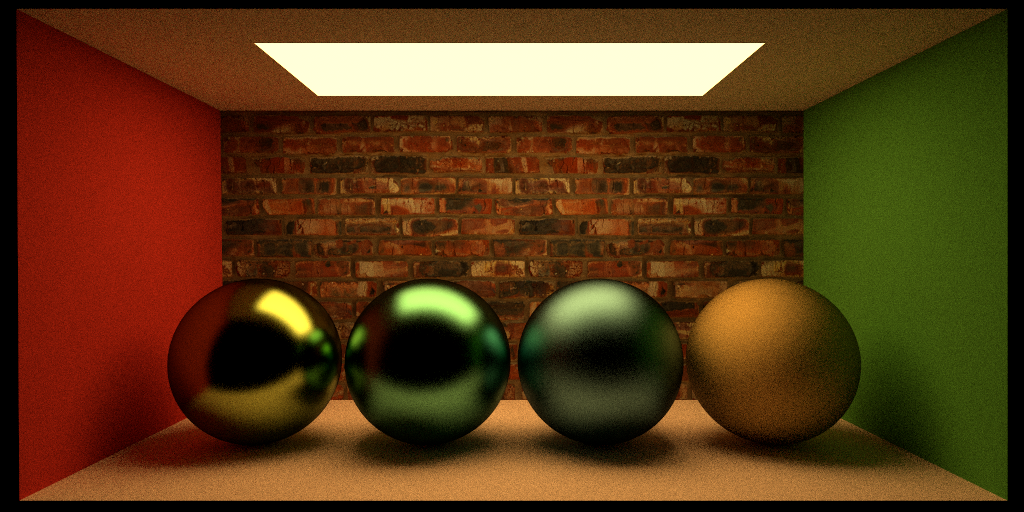
\includegraphics[width=0.45\linewidth]{imgs/hw_4_2f.png}
    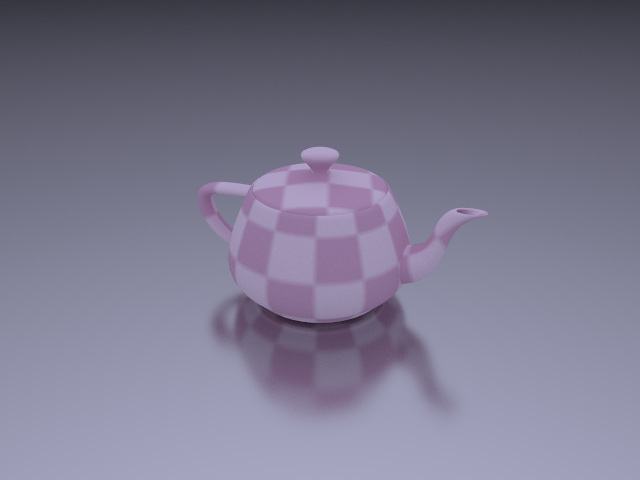
\includegraphics[width=0.225\linewidth]{imgs/hw_4_2g.png}
    \includegraphics[width=0.225\linewidth]{imgs/hw_4_2h.png}
    \caption{Reference for the \lstinline{blinnphong} materials for HW 4.2.}
    \label{fig:hw_4_2_blinn}
\end{figure}

\subsection{(Blinn-Phong) Microfacet BRDF}
The use of half vectors in the Blinn-Phong BRDF reveals an important physical insight.
Turns out we can build a geometrical/physical explanation of the idea of using half vectors to define BRDFs. The physical explanation is called \emph{Microfacet theory}.\footnote{Microfacet theory was developed in optical physics in 1960s by Beckmann anad Spizzchino to study electromagnectic wave scatter on surfaces. \href{https://www.graphics.cornell.edu/~westin/pubs/TorranceSparrowJOSA1967.pdf}{Torrance and Sparrow} then used similar theory to design microfacet BRDFs. \href{https://dl.acm.org/doi/10.1145/965141.563893}{Blinn} introduced the idea to graphics. \href{https://graphics.pixar.com/library/ReflectanceModel/paper.pdf}{Cook and Torrance} later wrote a more comprehensive introduction.} The idea is to treat the surface as a statistical collection of small oriented mirrors (and these mirrors are called the \emph{microfacets}). Mirrors only reflect lights when the half vector is aligned with its normal direction. So if we are reflecting light at half vector $h$, we must have hit a small mirror with \emph{micronormal} $m=h$. The half vector cosine lobe $\left(n_s \cdot h\right)^{\alpha}$ can be seen as defining a distribution of normals, by counting how many mirrors have the normal $h$. Each individual mirror also has its own Fresnel reflection, which is why we use half vector instead of shading normal for the Fresnel. Finally, the microfacets can block each other, causing shadowing effects. Mathematically, a microfacet BRDF is defined as:
\begin{equation}
\rho_{\text{microfacet}} = \begin{cases}
\frac{F_h \cdot D \cdot G}{4 \left(n_s \cdot \omega_i\right)} \text{ if } n_s \cdot \omega_o > 0 \\
0 & \text{ otherwise} 
\end{cases},
\label{eq:microfacet}
\end{equation}
where $F_h$ is the Fresnel term (we will use the Schlick Fresnel as in Equation~\eqref{eq:schilick_fresnel}) but evaluated at the half vector, $D$ is the \emph{Normal Distribution Function} (NDF) that describes the distribution of the normals of the microfacets, and $G$ is the geometric \emph{shadowing masking} term, which accounts for the porortion of unblocked microfacets. The $n_s \cdot \omega_i$ models the total projection area of microfacets towards incoming (if you look at a surface from the grazing angle, you will see more area). The $4$ in the denominator is a normalization constant for energy conservation.
Microfacet BRDFs are the most popular BRDFs in computer graphics now, because of how well they fit to our current BRDF datasets (see, again, the article by \href{http://people.csail.mit.edu/addy/research/brdf/index.html}{Ngan et al.} for more detail).

For $D$, we will use a Blinn-Phong inspired NDF:
\begin{equation}
D \propto \left(n_s \cdot h\right)^{\alpha}.
\label{eq:blinn_NDF}
\end{equation}
Notice how Equation~\eqref{eq:microfacet} is basically the Blinn-Phong BRDF but taking into account the microfacet projection area and occlusion.
The division of the projection area of microfacets is what will fix our darkening issue in Blinn-Phong!
$G$, on the other hand, is crucial for physical consistency.

$G$ can usually be derived from the geometric configuration of the microfacets. The most popular configuration is developed by \href{https://ieeexplore.ieee.org/document/1138991}{Smith}: they assume that the microfacets' orientations are uncorrelated to each other. With this assumption, the geometry term is a function solely on the two viewing directions: 
\begin{equation}
\begin{aligned}
G(\omega_i, \omega_o) &= G_1(\omega_i) G_1(\omega_o) \\
G_1(\omega) = \begin{cases}
0 & \text{ if } \omega \cdot h \leq 0 \\
\hat{G}_1(\omega) & \text{ otherwise.}
\end{cases}
\end{aligned}
\end{equation}
We can derive $G_1$ using the conservation of projection area of the microfacet:
\begin{equation}
\begin{aligned}
\omega \cdot n_s &= \int_{\Omega_h} G_1(\omega) D(h) \omega \cdot h \mathrm{d} h \\
G_1(\omega) &= \frac{\omega \cdot n_s}{\int_{\Omega_h} D(h) \omega \cdot h \mathrm{d} h}. 
\label{eq:smith_g1}
\end{aligned}
\end{equation}
(See \href{https://jcgt.org/published/0003/02/03/}{Understanding the Masking-Shadowing Function in Microfacet-Based BRDFs} for a comprehensive derivation).

Unfortunately, the integral in Equation~\eqref{eq:smith_g1} does not have a known closed-form for the Blinn-Phong NDF. We will use the rational polynomial fit from \href{http://www.graphics.cornell.edu/~bjw/microfacetbsdf.pdf}{Walter et al.} instead:
\begin{equation}
\begin{aligned}
a &= \frac{\sqrt{0.5 \alpha + 1}}{\tan\theta} \\
\hat{G}_1(\omega) &= \begin{cases}
\frac{3.535a + 2.181a^2}{1 + 2.276a + 2.577a^2} & \text{ if } a < 1.6 \\
1 & \text{ otherwise}
\end{cases}
\end{aligned}.
\end{equation}

Notice that our NDF (Equation~\eqref{eq:blinn_NDF}) is only defined up to a constant. Normalization of NDF is slightly different from normalizing the Phong BRDF. We, again, need to take the projection area of the microfacets into account:
\begin{equation}
\int_{\omega_h} D(h) n_s \cdot h \mathrm{d}h = 1.
\end{equation}
See \href{https://www.reedbeta.com/blog/hows-the-ndf-really-defined/}{this blog post} from Nathan Reed for a nice explanation. Fortunately, the integral above has a closed-form this time. Let $D(h) = C \left(n_s \cdot h\right)^{\alpha}$, the integral is exactly the same as Equation~\eqref{eq:phong_normalization}, so we get $C = \frac{\alpha + 2}{2\pi}$ again.

We can reuse the sampling procedure for sampling Blinn-Phong for sampling the Blinn-Phong microfacet BRDF. It does not importance sample $G$, but typically the BRDF is dominated by the $D$ term, so it is usually fine.\footnote{\href{https://hal.inria.fr/hal-00996995/en}{A paper} from Heitz and d'Eon discusses how to importance sample $D \cdot G$.}

Now, implement the Blinn-Phong microfacet BRDF in your \lstinline{hw_4_2} code. Our microfacet BRDF has the same parameters as a Phong BRDF:
\begin{lstlisting}[language=C++]
struct ParsedBlinnPhongMicrofacet {
    ParsedColor reflectance; // Ks
    Real exponent; // alpha
};
\end{lstlisting}

If we render the same scenes again (Figure~\ref{fig:hw_4_2_blinn_microfacet}):
\begin{lstlisting}[language=bash]
./torrey -hw 4_2 ../scenes/cbox/cbox_area_light_spheres_blinn_microfacet.xml
./torrey -hw 4_2 ../scenes/teapot/teapot_textured_blinn_microfacet.xml
./torrey -hw 4_2 ../scenes/teapot/teapot_textured_blinn_microfacet_grazing_view.xml
\end{lstlisting}
We will notice that the darkening issue is gone, and we reproduce the desired grazing angle behavior in the last scene!

\begin{figure}[ht]
    \centering
    \includegraphics[width=0.45\linewidth]{imgs/hw_4_2i.png}
    \includegraphics[width=0.225\linewidth]{imgs/hw_4_2j.png}
    \includegraphics[width=0.225\linewidth]{imgs/hw_4_2k.png}
    \caption{Reference for the \lstinline{blinn_microfacet} materials for HW 4.2.}
    \label{fig:hw_4_2_blinn_microfacet}
\end{figure}

\section{Multiple importance sampling}
It's time to add explicit light sampling (i.e. \emph{next event estimation}) from the previous homework back. Now at each shading point, we have two sampling strategies: one importance samples the BRDF, and the other one importance sample the light source. We will adopt \href{https://cseweb.ucsd.edu/~viscomp/classes/cse168/sp21/readings/veach.pdf}{Multiple Importance Sampling} (MIS) for combining the two strategies. In particular, we will adopt the \emph{one-sample} variant of MIS: instead of deterministically shooting rays for both lights and BRDFs and weighing them, we randomly choose one and combine the distribution. The deterministic version of MIS is usually more efficient (because of the stratification effect), but the one-sample variant fits much better to our current code and is easier to implement.

Read \href{https://raytracing.github.io/books/RayTracingTheRestOfYourLife.html#mixturedensities}{Chapter 10-12} of RTRYL and combine light sampling with BRDF sampling by blending their sampling distribution in your code. You should combine light sampling with the sampling procedures we implemented for \lstinline{diffuse}, \lstinline{plastic}, \lstinline{phong}, \lstinline{blinnphong}, and \lstinline{blinn_microfacet}. For \lstinline{mirror}, light sampling won't have any effect. Implement the code in \lstinline{hw_4_3}.

%\bibliographystyle{plain}
%\bibliography{refs}

\end{document}
